% THIS IS IPRESPROC-SP.TEX, A LIGHT MODIFICATION OF SIGPROC-SP THAT SIMPLIFIES
% FORMATTING, BALANCES ENDING COLUMNS, AND ADDS THE IPRES LICENSE BLOCK.
%
% THIS IS SIGPROC-SP.TEX - VERSION 3.1
% WORKS WITH V3.2SP OF ACM_PROC_ARTICLE-SP.CLS
% APRIL 2009
%
% It is an example file showing how to use the 'acm_proc_article-sp.cls' V3.2SP
% LaTeX2e document class file for Conference Proceedings submissions.
% ----------------------------------------------------------------------------------------------------------------
% This .tex file (and associated .cls V3.2SP) *DOES NOT* produce:
%       1) The Permission Statement
%       2) The Conference (location) Info information
%       3) The Copyright Line with ACM data
%       4) Page numbering
% ---------------------------------------------------------------------------------------------------------------
% It is an example which *does* use the .bib file (from which the .bbl file
% is produced).
% REMEMBER HOWEVER: After having produced the .bbl file,
% and prior to final submission,
% you need to 'insert'  your .bbl file into your source .tex file so as to provide
% ONE 'self-contained' source file.
%
% Questions regarding SIGS should be sent to
% Adrienne Griscti ---> griscti@acm.org
%
% Questions/suggestions regarding the guidelines, .tex and .cls files, etc. to
% Gerald Murray ---> murray@hq.acm.org
%
% For tracking purposes - this is V3.1SP - APRIL 2009

\documentclass{ipres_proc_article-sp}

\begin{document}

\title{LaTeX Template for iPRES 2015}

%
% You need the command \numberofauthors to handle the 'placement
% and alignment' of the authors beneath the title.
%
% For aesthetic reasons, we recommend 'three authors at a time'
% i.e. three 'name/affiliation blocks' be placed beneath the title.
%
% NOTE: You are NOT restricted in how many 'rows' of
% "name/affiliations" may appear. We just ask that you restrict
% the number of 'columns' to three.
%
% Because of the available 'opening page real-estate'
% we ask you to refrain from putting more than six authors
% (two rows with three columns) beneath the article title.
% More than six makes the first-page appear very cluttered indeed.
%
% Use the \alignauthor commands to handle the names
% and affiliations for an 'aesthetic maximum' of six authors.
% Add names, affiliations, addresses for
% the seventh etc. author(s) as the argument for the
% \additionalauthors command.
% These 'additional authors' will be output/set for you
% without further effort on your part as the last section in
% the body of your article BEFORE References or any Appendices.

\numberofauthors{3} %  in this sample file, there are a *total*
% of EIGHT authors. SIX appear on the 'first-page' (for formatting
% reasons) and the remaining two appear in the \additionalauthors section.
%
\author{
% You can go ahead and credit any number of authors here,
% e.g. one 'row of three' or two rows (consisting of one row of three
% and a second row of one, two or three).
%
% The command \alignauthor (no curly braces needed) should
% precede each author name, affiliation/snail-mail address and
% e-mail address. Additionally, tag each line of
% affiliation/address with \affaddr, and tag the
% e-mail address with \email.
%
% 1st. author
\alignauthor
1st Author\\
       \affaddr{1st author's affiliation}\\
       \affaddr{1st line of address}\\
       \affaddr{2nd line of address}\\
       \affaddr{Tel \# incl. country code}\\
       \email{1st author email}
% 2nd. author
\alignauthor
2nd Author\\
       \affaddr{1st author's affiliation}\\
       \affaddr{1st line of address}\\
       \affaddr{2nd line of address}\\
       \affaddr{Tel \# incl. country code}\\
       \email{2nd author email}
% 3rd. author
\alignauthor
3rd Author\\
       \affaddr{1st author's affiliation}\\
       \affaddr{1st line of address}\\
       \affaddr{2nd line of address}\\
       \affaddr{Tel \# incl. country code}\\
       \email{3rd author email}
%
%\and  % use '\and' if you need 'another row' of author names
%
}

% There's nothing stopping you putting the seventh, eighth, etc.
% author on the opening page (as the 'third row') but we ask,
% for aesthetic reasons that you place these 'additional authors'
% in the \additional authors block, viz.
%\additionalauthors{Additional authors: John Smith (The Th{\o}rv{\"a}ld Group,
%email: {\texttt{jsmith@affiliation.org}}) and Julius P.~Kumquat
%(The Kumquat Consortium, email: {\texttt{jpkumquat@consortium.net}}).}
%\date{30 July 1999}
% Just remember to make sure that the TOTAL number of authors
% is the number that will appear on the first page PLUS the
% number that will appear in the \additionalauthors section.

\maketitle
\begin{abstract}
In this paper, we describe the formatting guidelines for iPRES 2015
Proceedings.
\end{abstract}

\terms{Your general terms must be any of the following nine designated terms: Institutional
opportunities and challenges; Infrastructure opportunities and challenges; Frameworks for
digital preservation; Preservation strategies and workflows; Innovative practice;
Training and education.}

\keywords{Keywords are your own designated keywords.}

\section{Introduction}
The proceedings are the records of the conference. iPRES hopes to give
these conference by-products a single, high-quality appearance. To do
this, we ask that authors follow some simple guidelines. In essence,
we ask you to make your paper look exactly like this document. The
easiest way to do this is simply to start with this document and
replace the content with your own material.

\section{Page Size}
All material on each page should fit within a rectangle of 18 x 23.5 cm
(7 inches x 9.25 inches), centered on the page, beginning 1.9 cm (0.75 inch) from
the top of the page and ending with 2.54 cm (1 inch) from the bottom.
The right and left margins should be 1.9 cm (.75 inch).  The text should
be in two 8.45 cm (3.33 inches) columns with a .83 cm (.33 inch) gutter.

\section{Typeset Text}
\subsection{Normal or Body Text}
Please use a 9-point Times Roman font, or other Roman font with serifs,
as close as possible in appearance to Times Roman in which these
guidelines have been set. The goal is to have a 9-point text, as
you see here. Please use sans-serif or non-proportional fonts only
for special purposes, such as distinguishing source code text. If
Times Roman is not available, try the font named Computer Modern
Roman. On a Macintosh, use the font named Times.  Right margins
should be justified, not ragged.

\subsection{Title and Authors}
The title (Helvetica 18-point bold), authors' names (Helvetica 12-point)
and affiliations (Helvetica 10-point) run across the full width of
the page -- one column wide. We also recommend phone number (Helvetica
10-point) and e-mail address (Helvetica 12-point). See the top of
this page for three addresses. If only one address is needed, center
all address text. For two addresses, use two centered tabs, and so on.
For more than three authors, you may have to improvise.\footnote{If
necessary, you may place some address information in a footnote, or
in a named section at the end of your paper.}

\subsection{First page copyright notice}
Please leave 3.81 cm (1.5 inches) of blank text box at the bottom of the
left column of the first page for the copyright notice. (Note that the
LaTeX processor will produce this automatically for you using the 
provided .cls file; you should not need to modify it).

\subsection{Subsequent Pages}
For pages other than the first page, start at the top of the page, and
continue in double-column format.  The two columns on the last page
should be as close to equal length as possible.

\begin{table}
\centering
\caption{Table captions should be placed above the table}
\begin{tabular}{|c|c|c|c|} \hline
Graphics & Top & In-bewteen & Bottom \\ \hline
Tables & End & Last & First \\ \hline
Figures & Good & Similar & Very well \\ \hline
\end{tabular}
\end{table}

\begin{figure}
\centering
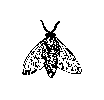
\epsfig{file=fly.eps}
\caption{A sample black and white graphic (.eps format).}
\end{figure}

\subsection{References and Citations}
Footnotes should be Times New Roman 9-point, and justified to the full
width of the column.

Use the ``Reference format'' for references -- that is, a numbered list
at the end of the article, ordered alphabetically and formatted
accordingly. See examples of some typical reference types, in the
new ``Reference format'', at the end of this document. Within this
template, use the style named references for the text. Acceptable
abbreviations, for journal names, can be found here:
\url{http://library.caltech.edu/reference/abbreviations/}. The correct style
for links in your references is NO underlining.

The references are also in 9 pt., but that section (see Section 7)
is ragged right. References should be published materials accessible
to the public. Internal technical reports may be cited only if they
are easily accessible (i.e. you can give the address to obtain the
report within your citation) and may be obtained by any reader.
Proprietary information may not be cited. Private communications should
be acknowledged, not referenced  (e.g., ``[Robertson, personal communication]'').

\textit{\LaTeX-specific notes:}

Citations to articles \cite{bowman:reasoning,
clark:pct, braams:babel, herlihy:methodology},
conference proceedings \cite{clark:pct} or
books \cite{salas:calculus, Lamport:LaTeX} listed
in the Bibliography section of your
article will occur throughout the text of your article.
You should use BibTeX to automatically produce this bibliography;
you simply need to insert one of several citation commands with
a key of the item cited in the proper location in
the \texttt{.tex} file \cite{Lamport:LaTeX}.

\section{Figures/Captions}
Place Tables/Figures/Images in text as close to the reference as possible
(see Figure 1).  It may extend across both columns to a maximum width
of 17.78 cm (7 inches). Captions should be Times New Roman 9-point bold.
They  should be numbered (e.g., ``Table 1'' or ``Figure 2''), please note that
the word for Table and Figure are spelled out. Figure's captions should
be centered beneath the image or picture, and Table captions should be
centered above the table body.

\subsection{Subsections}
The heading of subsections should be in Times New Roman 12-point bold
with only the initial letters capitalized. (Note: For subsections and
subsubsections, a word like \textit{the} or \textit{a} is not capitalized
unless it is the first word of the header.)

\subsubsection{Subsubsections}
The heading for subsubsections should be in Times New Roman 11-point
italic with initial letters capitalized and 6-points of white space
above the subsubsection head.

\subsubsection{Subsubsections}
The heading for subsubsections should be in Times New Roman 11-point
italic with initial letters capitalized.

\subsubsection{Subsubsections}
The heading for subsubsections should be in Times New Roman 11-point
italic with initial letters capitalized.

% Small space between end of paper body and acknowledgements. Remove if desired.
\vskip 1em

\section{Acknowledgements}
Our thanks to ACM for allowing us to modify templates they had developed.


%
% The following two commands are all you need in the
% initial runs of your .tex file to
% produce the bibliography for the citations in your paper.
\bibliographystyle{abbrv}
\bibliography{ipresproc}  % ipresproc.bib is the name of the Bibliography in this case
% You must have a proper ".bib" file
%  and remember to run:
% latex bibtex latex latex
% to resolve all references
%
% ACM needs 'a single self-contained file'!
% Generated by bibtex from your ~.bib file.  Run latex,
% then bibtex, then latex twice (to resolve references)
% to create the ~.bbl file.  Insert that ~.bbl file into
% the .tex source file and comment out
% the command \texttt{{\char'134}thebibliography}.
%

% \balancecolumns % Patched out for iPRES - using flushend instead
% That's all folks!
\end{document}
